\documentclass[border=8pt]{standalone}
\usepackage[T1]{fontenc}\usepackage{helvet}\renewcommand{\familydefault}{\sfdefault}
\usepackage{tikz}\usetikzlibrary{arrows.meta, positioning, calc, backgrounds}
\definecolor{ink}{HTML}{1a1916}
\definecolor{inktwo}{HTML}{3a3a35}
\definecolor{inkthree}{HTML}{6a6862}
\definecolor{rule}{HTML}{b8b09a}
\definecolor{amber}{HTML}{a8730a}
\definecolor{red}{HTML}{c8261a}
\definecolor{paper}{HTML}{f0eee5}
\definecolor{slab}{HTML}{d8d4c6}
\tikzset{
  >={Stealth[length=2.2mm]},
  wire/.style={line width=0.8pt, ink},
  modwire/.style={line width=0.6pt, dashed, ink},
  tastewire/.style={line width=0.6pt, dashed, amber},
  gatewire/.style={line width=0.6pt, dotted, ink},
  block/.style={rectangle, draw=ink, line width=0.9pt, fill=slab, minimum width=2.4cm, minimum height=1.9cm, inner sep=0pt},
  perf/.style={rectangle, draw=ink, line width=0.7pt, minimum width=2.4cm, minimum height=0.7cm, inner sep=2pt, font=\footnotesize, text=ink},
  title/.style={font=\footnotesize\bfseries, text=ink, anchor=north, inner sep=2pt},
  jack/.style={circle, draw=ink, fill=paper, line width=0.5pt, minimum size=3.2pt, inner sep=0pt},
  plabel/.style={font=\tiny, text=inktwo, anchor=west, inner sep=1pt},
  olabel/.style={font=\tiny, text=inktwo, anchor=east, inner sep=1pt},
  settings/.style={font=\scriptsize, text=ink, align=left, anchor=north west, inner sep=1pt, text width=2.3cm},
}
\begin{document}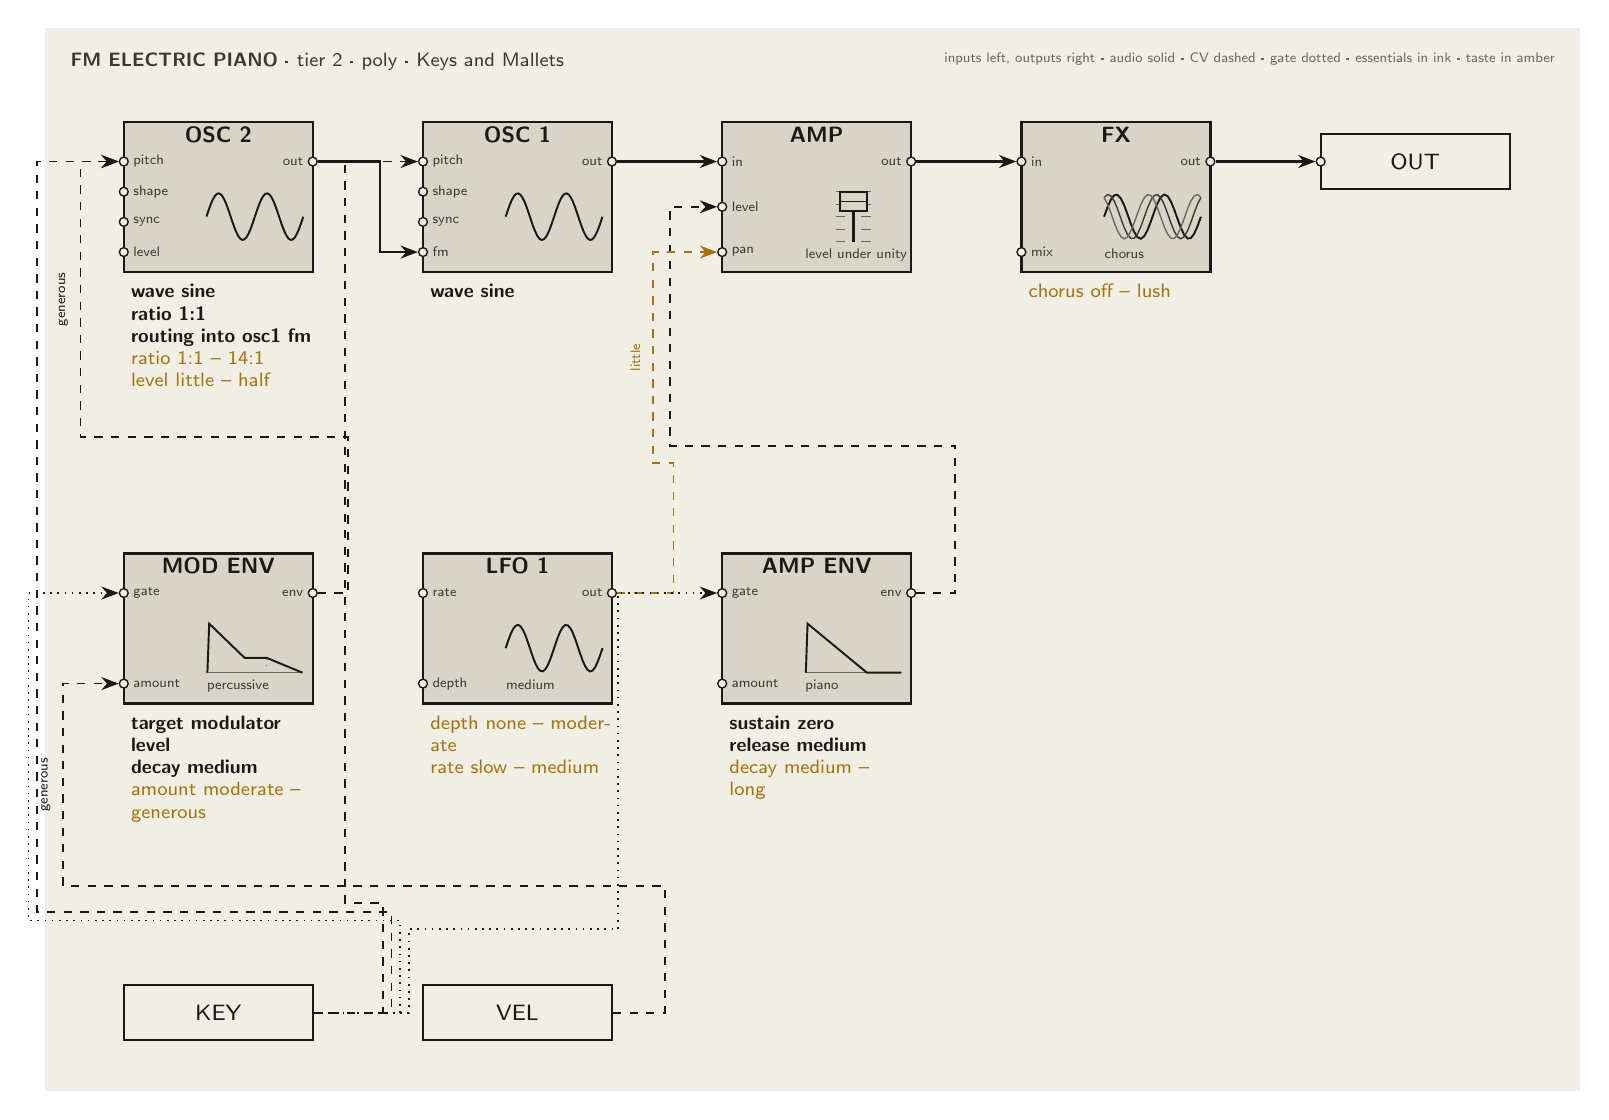
\begin{tikzpicture}
\begin{scope}[on background layer]\fill[paper] (-2.2,-11.36) rectangle (17.299999999999997,2.15);\end{scope}
\node[block, minimum height=1.9cm] (osc1) at (3.8,0.0) {};
\node[title] at (osc1.north) {OSC 1};
\node[jack] (osc1-pitch) at (2.5999999999999996,0.44999999999999996) {};
\node[plabel] at (2.6799999999999997,0.44999999999999996) {pitch};
\node[jack] (osc1-shape) at (2.5999999999999996,0.06666666666666665) {};
\node[plabel] at (2.6799999999999997,0.06666666666666665) {shape};
\node[jack] (osc1-sync) at (2.5999999999999996,-0.31666666666666665) {};
\node[plabel] at (2.6799999999999997,-0.31666666666666665) {sync};
\node[jack] (osc1-fm) at (2.5999999999999996,-0.7) {};
\node[plabel] at (2.6799999999999997,-0.7) {fm};
\node[jack] (osc1-out) at (5.0,0.44999999999999996) {};
\node[olabel] at (4.92,0.44999999999999996) {out};
\begin{scope}
\draw[ink, line width=0.7pt] plot[domain=0.000:0.500, samples=24, variable=\u] ({3.650+\u*1.230},{-0.620+(0.740)*(0.5+0.4*sin(360*(\u*2))+0.0)});
\draw[ink, line width=0.7pt] plot[domain=0.500:1.000, samples=24, variable=\u] ({3.650+\u*1.230},{-0.620+(0.740)*(0.5+0.4*sin(360*(\u*2))+0.0)});
\end{scope}
\node[settings] at (2.6499999999999995,-1.0699999999999998) {\textbf{wave sine}};
\node[block, minimum height=1.9cm] (osc2) at (0.0,0.0) {};
\node[title] at (osc2.north) {OSC 2};
\node[jack] (osc2-pitch) at (-1.2,0.44999999999999996) {};
\node[plabel] at (-1.1199999999999999,0.44999999999999996) {pitch};
\node[jack] (osc2-shape) at (-1.2,0.06666666666666665) {};
\node[plabel] at (-1.1199999999999999,0.06666666666666665) {shape};
\node[jack] (osc2-sync) at (-1.2,-0.31666666666666665) {};
\node[plabel] at (-1.1199999999999999,-0.31666666666666665) {sync};
\node[jack] (osc2-level) at (-1.2,-0.7) {};
\node[plabel] at (-1.1199999999999999,-0.7) {level};
\node[jack] (osc2-out) at (1.2,0.44999999999999996) {};
\node[olabel] at (1.1199999999999999,0.44999999999999996) {out};
\begin{scope}
\draw[ink, line width=0.7pt] plot[domain=0.000:0.500, samples=24, variable=\u] ({-0.150+\u*1.230},{-0.620+(0.740)*(0.5+0.4*sin(360*(\u*2))+0.0)});
\draw[ink, line width=0.7pt] plot[domain=0.500:1.000, samples=24, variable=\u] ({-0.150+\u*1.230},{-0.620+(0.740)*(0.5+0.4*sin(360*(\u*2))+0.0)});
\end{scope}
\node[settings] at (-1.15,-1.0699999999999998) {\textbf{wave sine} \\ \textbf{ratio 1:1} \\ \textbf{routing into osc1 fm} \\ \textcolor{amber}{ratio 1:1 -- 14:1} \\ \textcolor{amber}{level little -- half}};
\node[block, minimum height=1.9cm] (amp) at (7.6,0.0) {};
\node[title] at (amp.north) {AMP};
\node[jack] (amp-in) at (6.3999999999999995,0.44999999999999996) {};
\node[plabel] at (6.4799999999999995,0.44999999999999996) {in};
\node[jack] (amp-level) at (6.3999999999999995,-0.125) {};
\node[plabel] at (6.4799999999999995,-0.125) {level};
\node[jack] (amp-pan) at (6.3999999999999995,-0.7) {};
\node[plabel] at (6.4799999999999995,-0.7) {pan};
\node[jack] (amp-out) at (8.799999999999999,0.44999999999999996) {};
\node[olabel] at (8.719999999999999,0.44999999999999996) {out};
\begin{scope}
\draw[ink, line width=1.2pt] (8.065,-0.570) -- (8.065,0.070);
\draw[inkthree, line width=0.3pt] (7.845,-0.570) -- (7.965,-0.570) (8.165,-0.570) -- (8.285,-0.570);
\draw[inkthree, line width=0.3pt] (7.845,-0.410) -- (7.965,-0.410) (8.165,-0.410) -- (8.285,-0.410);
\draw[inkthree, line width=0.3pt] (7.845,-0.250) -- (7.965,-0.250) (8.165,-0.250) -- (8.285,-0.250);
\draw[inkthree, line width=0.3pt] (7.845,-0.090) -- (7.965,-0.090) (8.165,-0.090) -- (8.285,-0.090);
\draw[inkthree, line width=0.3pt] (7.845,0.070) -- (7.965,0.070) (8.165,0.070) -- (8.285,0.070);
\fill[slab, draw=ink, line width=0.6pt] (7.895,-0.178) rectangle (8.235,0.062);
\draw[ink, line width=0.5pt] (7.895,-0.058) -- (8.235,-0.058);
\node[font=\tiny, text=inktwo, anchor=north west, inner sep=0pt] at (7.450,-0.650) {level under unity};
\end{scope}
\node[block, minimum height=1.9cm] (fx) at (11.399999999999999,0.0) {};
\node[title] at (fx.north) {FX};
\node[jack] (fx-in) at (10.2,0.44999999999999996) {};
\node[plabel] at (10.28,0.44999999999999996) {in};
\node[jack] (fx-mix) at (10.2,-0.7) {};
\node[plabel] at (10.28,-0.7) {mix};
\node[jack] (fx-out) at (12.599999999999998,0.44999999999999996) {};
\node[olabel] at (12.519999999999998,0.44999999999999996) {out};
\begin{scope}
\draw[ink, line width=0.7pt] plot[domain=0.000:1.000, samples=30, variable=\u] ({11.250+\u*1.230},{-0.620+(0.740)*(0.5+0.38*sin(360*((\u-0.000)/1.000)*2+0))});
\draw[inktwo, line width=0.5pt] plot[domain=0.000:1.000, samples=30, variable=\u] ({11.250+\u*1.230},{-0.620+(0.740)*(0.5+0.38*sin(360*((\u-0.000)/1.000)*2+60))});
\draw[inkthree, line width=0.5pt] plot[domain=0.000:1.000, samples=30, variable=\u] ({11.250+\u*1.230},{-0.620+(0.740)*(0.5+0.38*sin(360*((\u-0.000)/1.000)*2+120))});
\node[font=\tiny, text=inktwo, anchor=north west, inner sep=0pt] at (11.250,-0.650) {chorus};
\end{scope}
\node[settings] at (10.25,-1.0699999999999998) {\textcolor{amber}{chorus off -- lush}};
\node[block, minimum height=1.9cm] (menv) at (0.0,-5.4799999999999995) {};
\node[title] at (menv.north) {MOD ENV};
\node[jack] (menv-gate) at (-1.2,-5.029999999999999) {};
\node[plabel] at (-1.1199999999999999,-5.029999999999999) {gate};
\node[jack] (menv-amount) at (-1.2,-6.18) {};
\node[plabel] at (-1.1199999999999999,-6.18) {amount};
\node[jack] (menv-out) at (1.2,-5.029999999999999) {};
\node[olabel] at (1.1199999999999999,-5.029999999999999) {env};
\begin{scope}
\draw[inkthree, line width=0.3pt] (-0.150,-6.041) -- (1.080,-6.041);
\draw[ink, line width=0.7pt] (-0.138,-6.041) -- (-0.115,-5.419) -- (0.335,-5.854) -- (0.617,-5.854) -- (1.068,-6.041);
\draw[inkthree, line width=0.3pt, dotted] (0.617,-6.041) -- (0.617,-5.854);
\node[font=\tiny, text=inktwo, anchor=north west, inner sep=0pt] at (-0.150,-6.130) {percussive};
\end{scope}
\node[settings] at (-1.15,-6.55) {\textbf{target modulator level} \\ \textbf{decay medium} \\ \textcolor{amber}{amount moderate -- generous}};
\node[block, minimum height=1.9cm] (lfo1) at (3.8,-5.4799999999999995) {};
\node[title] at (lfo1.north) {LFO 1};
\node[jack] (lfo1-rate) at (2.5999999999999996,-5.029999999999999) {};
\node[plabel] at (2.6799999999999997,-5.029999999999999) {rate};
\node[jack] (lfo1-depth) at (2.5999999999999996,-6.18) {};
\node[plabel] at (2.6799999999999997,-6.18) {depth};
\node[jack] (lfo1-out) at (5.0,-5.029999999999999) {};
\node[olabel] at (4.92,-5.029999999999999) {out};
\begin{scope}
\draw[ink, line width=0.7pt] plot[domain=0:1, samples=40, variable=\u] ({3.650+\u*1.230},{-6.100+(0.740)*(0.5+0.4*sin(360*\u*2))});
\node[font=\tiny, text=inktwo, anchor=north west, inner sep=0pt] at (3.650,-6.130) {medium};
\end{scope}
\node[settings] at (2.6499999999999995,-6.55) {\textcolor{amber}{depth none -- moderate} \\ \textcolor{amber}{rate slow -- medium}};
\node[block, minimum height=1.9cm] (aenv) at (7.6,-5.4799999999999995) {};
\node[title] at (aenv.north) {AMP ENV};
\node[jack] (aenv-gate) at (6.3999999999999995,-5.029999999999999) {};
\node[plabel] at (6.4799999999999995,-5.029999999999999) {gate};
\node[jack] (aenv-amount) at (6.3999999999999995,-6.18) {};
\node[plabel] at (6.4799999999999995,-6.18) {amount};
\node[jack] (aenv-out) at (8.799999999999999,-5.029999999999999) {};
\node[olabel] at (8.719999999999999,-5.029999999999999) {env};
\begin{scope}
\draw[inkthree, line width=0.3pt] (7.450,-6.041) -- (8.680,-6.041);
\draw[ink, line width=0.7pt] (7.462,-6.041) -- (7.484,-5.419) -- (8.237,-6.041) -- (8.237,-6.041) -- (8.668,-6.041);
\node[font=\tiny, text=inktwo, anchor=north west, inner sep=0pt] at (7.450,-6.130) {piano};
\end{scope}
\node[settings] at (6.449999999999999,-6.55) {\textbf{sustain zero} \\ \textbf{release medium} \\ \textcolor{amber}{decay medium -- long}};
\node[perf] (key) at (0.0,-10.36) {KEY};
\node[perf] (vel) at (3.8,-10.36) {VEL};
\node[perf, fill=paper] (out) at (15.2,0.44999999999999996) {OUT}; \node[jack] (out-in) at (14.0,0.44999999999999996) {};
\draw[wire,->] (osc2-out) -- (2.05,0.44999999999999996) -- (2.05,-0.7) -- (osc1-fm);
\draw[wire,->] (osc1-out) -- (amp-in);
\draw[wire,->] (amp-out) -- (fx-in);
\draw[wire,->] (fx-out) -- (out-in);
\draw[modwire,->] (menv-out) -- (1.65,-5.029999999999999) -- (1.65,-3.05) -- (-1.75,-3.05) -- (-1.75,0.44999999999999996) -- (osc2-pitch);
\node[font=\tiny, text=ink, anchor=south, inner sep=1pt, rotate=90] at (-1.87,-1.2999999999999998) {generous};
\draw[modwire,->] (aenv-out) -- (9.359999999999998,-5.029999999999999) -- (9.359999999999998,-3.1599999999999997) -- (5.739999999999999,-3.1599999999999997) -- (5.739999999999999,-0.125) -- (amp-level);
\draw[modwire,->] (vel.east) -- (5.67,-10.36) -- (5.67,-8.75) -- (-1.97,-8.75) -- (-1.97,-6.18) -- (menv-amount);
\node[font=\tiny, text=ink, anchor=south, inner sep=1pt, rotate=90] at (-2.09,-7.465) {generous};
\draw[tastewire,->] (lfo1-out) -- (5.78,-5.029999999999999) -- (5.78,-3.38) -- (5.52,-3.38) -- (5.52,-0.7) -- (amp-pan);
\node[font=\tiny, text=amber, anchor=south, inner sep=1pt, rotate=90] at (5.3999999999999995,-2.04) {little};
\draw[modwire,->] (key.east) -- (2.09,-10.36) -- (2.09,-8.969999999999999) -- (1.6099999999999999,-8.969999999999999) -- (1.6099999999999999,0.44999999999999996) -- (osc1-pitch);
\draw[modwire,->] (key.east) -- (2.2,-10.36) -- (2.2,-9.08) -- (-2.3,-9.08) -- (-2.3,0.44999999999999996) -- (osc2-pitch);
\draw[gatewire,->] (key.east) -- (2.31,-10.36) -- (2.31,-9.19) -- (-2.41,-9.19) -- (-2.41,-5.029999999999999) -- (menv-gate);
\draw[gatewire,->] (key.east) -- (2.42,-10.36) -- (2.42,-9.299999999999999) -- (5.08,-9.299999999999999) -- (5.08,-5.029999999999999) -- (aenv-gate);
\node[anchor=north west, font=\scriptsize, text=inktwo] at (-2.0,1.95) {\textbf{FM ELECTRIC PIANO} · tier 2 · poly · Keys and Mallets};
\node[anchor=north east, font=\tiny, text=inkthree] at (17.099999999999998,1.95) {inputs left, outputs right · audio solid · CV dashed · gate dotted · essentials in ink · taste in amber};
\end{tikzpicture}\end{document}
